\documentclass{article}\usepackage[]{graphicx}\usepackage[]{xcolor}
% maxwidth is the original width if it is less than linewidth
% otherwise use linewidth (to make sure the graphics do not exceed the margin)
\makeatletter
\def\maxwidth{ %
  \ifdim\Gin@nat@width>\linewidth
    \linewidth
  \else
    \Gin@nat@width
  \fi
}
\makeatother

\definecolor{fgcolor}{rgb}{0.345, 0.345, 0.345}
\newcommand{\hlnum}[1]{\textcolor[rgb]{0.686,0.059,0.569}{#1}}%
\newcommand{\hlstr}[1]{\textcolor[rgb]{0.192,0.494,0.8}{#1}}%
\newcommand{\hlcom}[1]{\textcolor[rgb]{0.678,0.584,0.686}{\textit{#1}}}%
\newcommand{\hlopt}[1]{\textcolor[rgb]{0,0,0}{#1}}%
\newcommand{\hlstd}[1]{\textcolor[rgb]{0.345,0.345,0.345}{#1}}%
\newcommand{\hlkwa}[1]{\textcolor[rgb]{0.161,0.373,0.58}{\textbf{#1}}}%
\newcommand{\hlkwb}[1]{\textcolor[rgb]{0.69,0.353,0.396}{#1}}%
\newcommand{\hlkwc}[1]{\textcolor[rgb]{0.333,0.667,0.333}{#1}}%
\newcommand{\hlkwd}[1]{\textcolor[rgb]{0.737,0.353,0.396}{\textbf{#1}}}%
\let\hlipl\hlkwb

\usepackage{framed}
\makeatletter
\newenvironment{kframe}{%
 \def\at@end@of@kframe{}%
 \ifinner\ifhmode%
  \def\at@end@of@kframe{\end{minipage}}%
  \begin{minipage}{\columnwidth}%
 \fi\fi%
 \def\FrameCommand##1{\hskip\@totalleftmargin \hskip-\fboxsep
 \colorbox{shadecolor}{##1}\hskip-\fboxsep
     % There is no \\@totalrightmargin, so:
     \hskip-\linewidth \hskip-\@totalleftmargin \hskip\columnwidth}%
 \MakeFramed {\advance\hsize-\width
   \@totalleftmargin\z@ \linewidth\hsize
   \@setminipage}}%
 {\par\unskip\endMakeFramed%
 \at@end@of@kframe}
\makeatother

\definecolor{shadecolor}{rgb}{.97, .97, .97}
\definecolor{messagecolor}{rgb}{0, 0, 0}
\definecolor{warningcolor}{rgb}{1, 0, 1}
\definecolor{errorcolor}{rgb}{1, 0, 0}
\newenvironment{knitrout}{}{} % an empty environment to be redefined in TeX

\usepackage{alltt}
\IfFileExists{upquote.sty}{\usepackage{upquote}}{}
\begin{document}

\begin{knitrout}
\definecolor{shadecolor}{rgb}{0.969, 0.969, 0.969}\color{fgcolor}\begin{kframe}
\begin{alltt}
\hlkwd{library}\hlstd{(sf)}
\end{alltt}


{\ttfamily\noindent\itshape\color{messagecolor}{\#\# Linking to GEOS 3.11.2, GDAL 3.7.2, PROJ 9.3.0; sf\_use\_s2() is TRUE}}\begin{alltt}
\hlkwd{library}\hlstd{(ggplot2)}
\hlkwd{library}\hlstd{(dplyr)}
\end{alltt}


{\ttfamily\noindent\itshape\color{messagecolor}{\#\# \\\#\# Attaching package: 'dplyr'}}

{\ttfamily\noindent\itshape\color{messagecolor}{\#\# The following objects are masked from 'package:stats':\\\#\# \\\#\# \ \ \ \ filter, lag}}

{\ttfamily\noindent\itshape\color{messagecolor}{\#\# The following objects are masked from 'package:base':\\\#\# \\\#\# \ \ \ \ intersect, setdiff, setequal, union}}\end{kframe}
\end{knitrout}

\begin{knitrout}
\definecolor{shadecolor}{rgb}{0.969, 0.969, 0.969}\color{fgcolor}\begin{kframe}
\begin{alltt}
\hlcom{# Load the shapefile}
\hlstd{london_boroughs} \hlkwb{<-} \hlkwd{st_read}\hlstd{(}\hlstr{"London_Ward.shp"}\hlstd{)}
\end{alltt}
\begin{verbatim}
## Reading layer `London_Ward' from data source 
##   `C:\Users\chuyu\Desktop\Data-Visualisation-Project\Test folder-Yujie Chu\London_Ward.shp' 
##   using driver `ESRI Shapefile'
## Simple feature collection with 657 features and 6 fields
## Geometry type: POLYGON
## Dimension:     XY
## Bounding box:  xmin: 503568.2 ymin: 155850.8 xmax: 561957.5 ymax: 200933.9
## Projected CRS: OSGB36 / British National Grid
\end{verbatim}
\begin{alltt}
\hlcom{# Load the crime data (assuming it's in CSV format)}
\hlstd{crime_data} \hlkwb{<-} \hlkwd{read.csv}\hlstd{(}\hlstr{"BoroughLevelCrime.csv"}\hlstd{)}

\hlcom{# Summing the total crimes for each borough over the entire timeframe}
\hlstd{borough_totals} \hlkwb{<-} \hlstd{crime_data} \hlopt
  \hlkwd{group_by}\hlstd{(LookUp_BoroughName)} \hlopt
  \hlkwd{summarise}\hlstd{(}\hlkwc{Total_Crimes} \hlstd{=} \hlkwd{sum}\hlstd{(}\hlkwd{across}\hlstd{(}\hlkwd{starts_with}\hlstd{(}\hlstr{"X2020"}\hlstd{))))}

\hlcom{# Merge the crime data with the shapefile}
\hlstd{merged_data} \hlkwb{<-} \hlkwd{merge}\hlstd{(london_boroughs, borough_totals,} \hlkwc{by.x}\hlstd{=}\hlstr{"DISTRICT"}\hlstd{,} \hlkwc{by.y}\hlstd{=}\hlstr{"LookUp_BoroughName"}\hlstd{)}

\hlcom{# Plot the merged data}
\hlstd{plot} \hlkwb{<-} \hlkwd{ggplot}\hlstd{(}\hlkwc{data}\hlstd{=merged_data)} \hlopt{+}
  \hlkwd{geom_sf}\hlstd{(}\hlkwd{aes}\hlstd{(}\hlkwc{fill}\hlstd{=Total_Crimes))} \hlopt{+}
  \hlkwd{scale_fill_gradient}\hlstd{(}\hlkwc{low}\hlstd{=}\hlstr{"Green"}\hlstd{,} \hlkwc{high}\hlstd{=}\hlstr{"red"}\hlstd{)} \hlopt{+}
  \hlkwd{theme_minimal}\hlstd{()} \hlopt{+}
  \hlkwd{labs}\hlstd{(}\hlkwc{title}\hlstd{=}\hlstr{"Total Crime by Borough in London (2020)"}\hlstd{,} \hlkwc{fill}\hlstd{=}\hlstr{"Total Crimes"}\hlstd{)}

\hlkwd{print}\hlstd{(plot)}
\end{alltt}
\end{kframe}
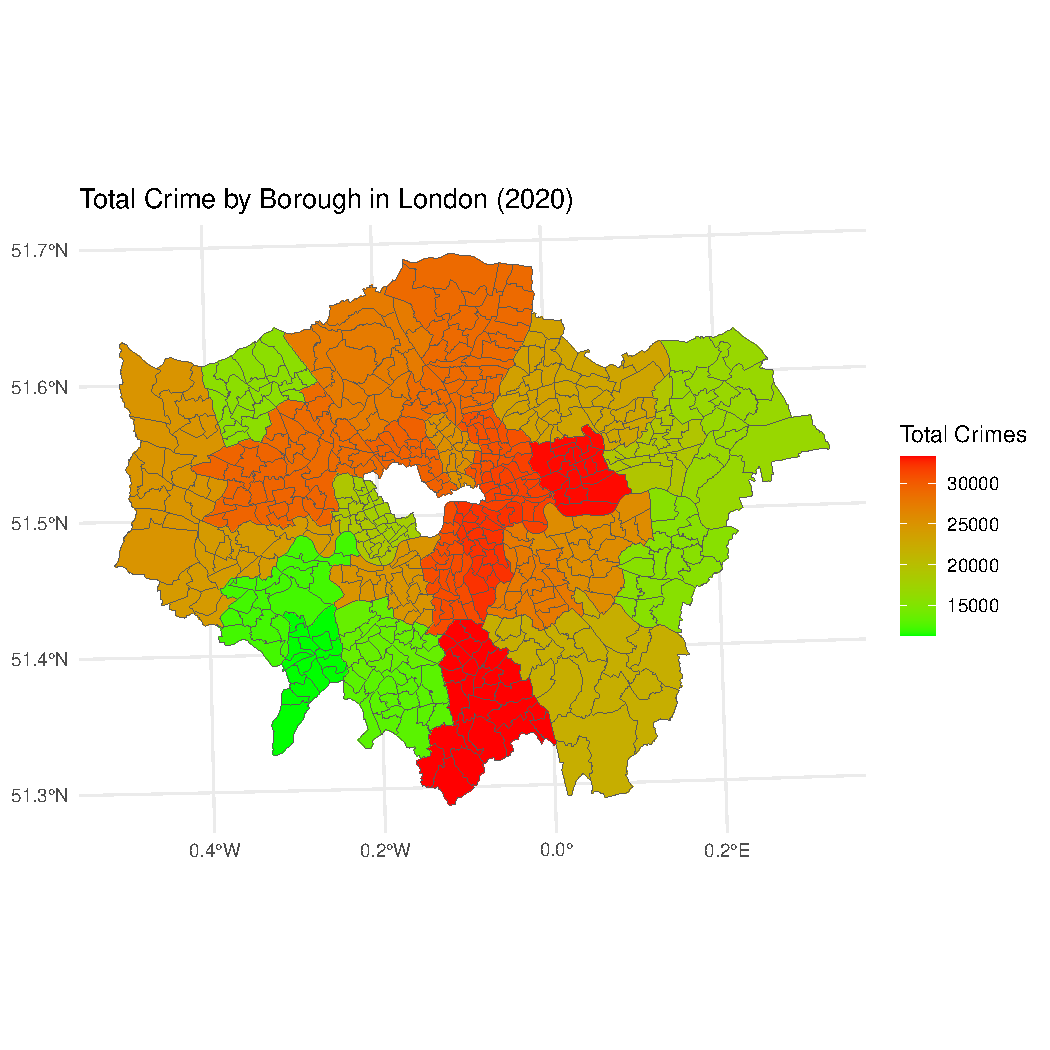
\includegraphics[width=\maxwidth]{figure/unnamed-chunk-1-1} 
\end{knitrout}




\end{document}
